\documentclass[a4paper, 12pt]{article}

\usepackage[portuges]{babel}
\usepackage[utf8]{inputenc}
\usepackage{indentfirst}
\usepackage{graphicx}
\usepackage{float}
\usepackage{listings}




\begin{document}

\begin{titlepage}
	\begin{center}
		\Huge{Processamento de Linguagens e Compiladores}\\
		\large{Universidade do Minho}\\
		\large{Ciências da Computação}\\ 
		\large{Trabalho Prático 1}\\ 
		\vspace{15pt}
        \vspace{95pt}
        \textbf{\LARGE{Processador de Pessoas Listadas em Róis de Confessados}}\\
		\vspace{3,5cm}
		\large{João Pedro Carvalho Henriques}\\
		\large{A81705}\\
		\vspace{3 cm}
		\large{2022}
	\end{center}	
\end{titlepage}

\tableofcontents

\newpage
\section{Introdução}\label{sec:intro}
O seguinte relatório foi realizado no âmbito da disciplia de Processamento de Linguagens e Compiladores onde são expostas todas as decisões tomadas na realização do trabalho prático.

O trabalho consiste no desenvolvimento de filtros de texto para extrair informação de um ficheiro de texto e tem como objetivo consolidar a aprendizagem da utilização de linguagens regulares em programas usando o módulo "re" do Python.

\newpage
\section{Problema}

\subsection{Descrição do problema}
Construa agora um ou vários programas Python para processar o texto 'processos.txt' com o intuito de calcular frequências de alguns elementos (a ideia é utilizar arrays associativos para o efeito) conforme solicitado a seguir:\\

a) Calcula a frequência de processos por ano (primeiro elemento da data);\\

b) Calcula a frequência de nomes próprios (o primeiro em cada nome) e apelidos (o ultimo em cada nome) por séculos;\\

c) Calcula a frequência dos vários tipos de relação: irmão, sobrinho, etc.\\

d) imprimir os 20 primeiros registos num novo ficheiro de output mas em formato Json.
\newpage
\subsection{Análise e Abordagem ao problema}
Após uma breve leitura do ficheiro processos.txt é possível observar que cada linha do ficheiro contém vários campos de informação separados por '::'.
Analisando várias linhas foi possível verificar a existência de um padrão. Esse padrão pode ser definido pelos seguintes campos: número, data, nome, nome do pai, nome da mãe e informação adicional. 

Após esta análise, já é possivel fazer uma abordagem mais concreta na resolução das alíneas. Podemos concluir que,  '::' antecede aos nomes próprios e procede aos apelidos, os nomes que aparecem no campo da informação adicional não foram contabilizados. As relações aparecem no campo da informação adicional sempre precedidas por uma vírgula. 

Assim,foi criado um menu inicial que permite ao utilizador escolher qual das alíneas pretende ver.Também foi criado um ficheiro de teste, teste.txt, correspondente às primeiras 30 linhas do ficheiro processos.txt, para testar as funções definidas na resolução das alíneas.  

Para facilitar a visualização da informação foram desenvolvidas duas funções em Python que atravès de um dicionario criam um ficheiro em HTML de uma tabela com a informação do dicionario.

Este projeto é constiuído por 2 ficheiros Python. O ficheiro func.py onde estão todas as funções necessárias para a resolução das alíneas e para a criação do ficheiro HTML e o ficheiro main.py onde está a implementação do menu inicial e onde são invocadas as funções.
\newpage
\section{Decisões tomadas e Exemplo de teste}
Nesta secção vão ser explicadas as decisões tomadas na implementação do código e o resultado da aplicação ao ficheiro teste.txt
\subsection{Frequência de processos por ano}
Para a resolução da primeira alínea foi utilizado um dicionário, associando a cada ano o número de processos registados. Assim, foi iterado sobre cada linha do ficheiro, e usando a função \textbf{search()} e a expressão regular \textbf{([0-9]{4})-([0-9]{2})-([0-9]{2})} foi possivel identificar a data e associar o primeiro grupo ao ano (ano = data.group(1)). Também foi feita a verificação para contabilizar linhas com número de processo e data iguais apenas uma vez.
\begin{figure}[H]
    \centering
    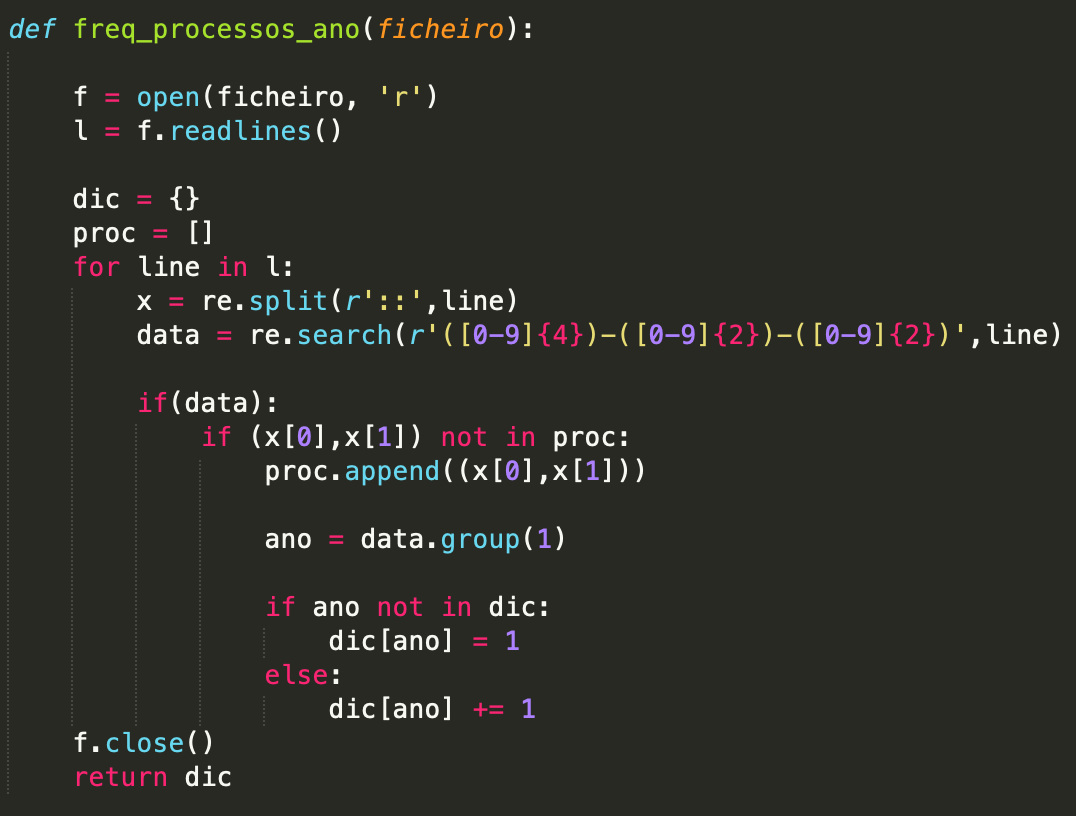
\includegraphics[height=3in]{freq_processos_ano.png}
    \caption[Optional caption]{Frequênica de processos por ano}
    \label{fig:my_label}
\end{figure}
\begin{figure}[H]
    \centering
    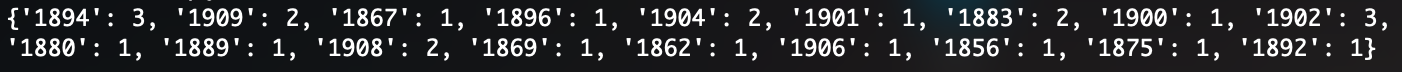
\includegraphics[height=0.3in]{freq_ano-teste.png}
    \caption{Exemplo de teste, Frequência de processos por ano}
    \label{fig:my_label}
\end{figure}
\begin{figure}[H]
    \centering
    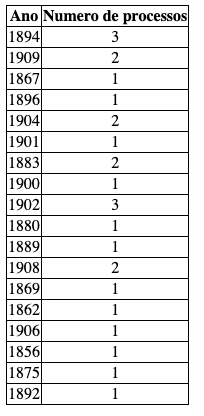
\includegraphics[height=3in]{freq_ano-tabela.png}
    \caption{Tabela de teste, Frequência de processos por ano}
    \label{fig:my_label}
\end{figure}
\newpage
\subsection{Frequência de nomes próprios e apelidos por século}
Na resolução da segunda alínea, o problema é divido em duas subalíneas, uma que calcula a frequência de nomes próprios por século e outra a frequência de apelidos por século
\subsubsection{Frequência de nomes próprios por século}
Para calcular a frequência de cada nome próprio por século foi também utilizado um dicionário que atribui a cada século outro dicionário que, por sua vez, atribui ao primeiro nome de cada nome a sua frequência,no respetivo século. Foi iterado sobre cada linha do ficheiro, onde através da expressão regular \textbf{'([A-Za-z]+)([ ][A-Za-z]+)*(\,[A-Za-z]+)?', r'$\backslash$1'} e da função \textbf{sub()}, todos os nomes completos são subtituidos pelo primeiro nome, e através da função \textbf{split()} aplicada ao resultado da ação anterior foi possivel guardar todos os campos separados por \textbf{'::'}. Assim os campos referentes ao nome, nome do pai e nome da mãe contêm apenas o primeiro nome. 
\begin{figure}[H]
    \centering
    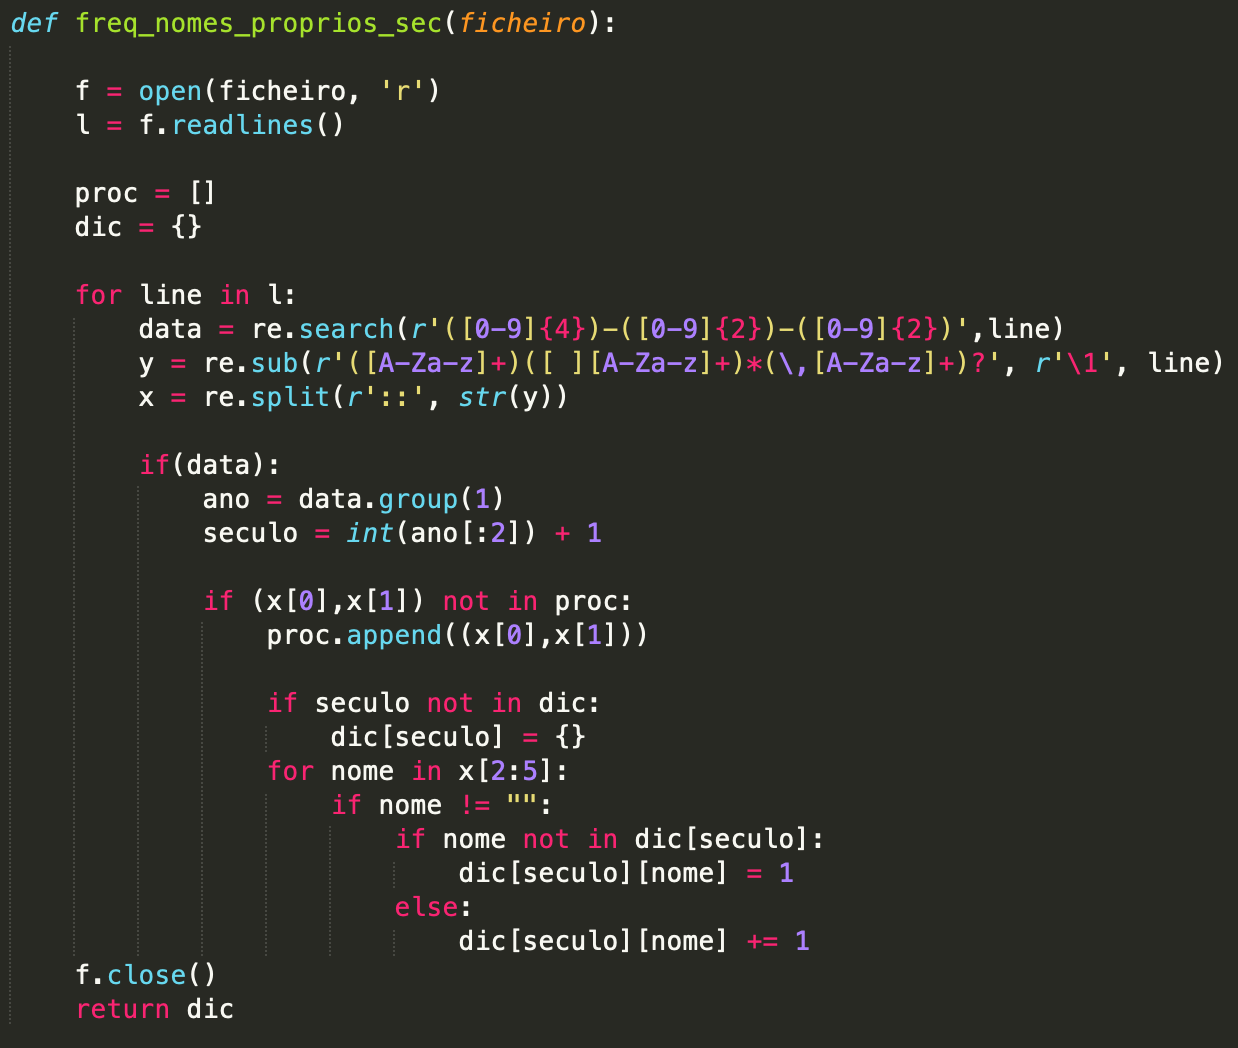
\includegraphics[height=3in]{freq_proprios_sec.png}
    \caption{Frequência de nomes próprios por século}
    \label{fig:my_label}
\end{figure}
\begin{figure}[H]
    \centering
    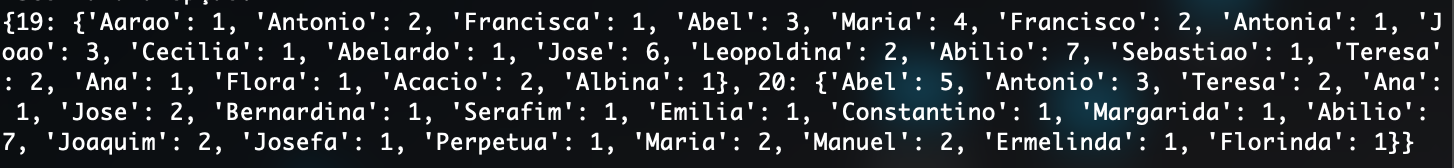
\includegraphics[height=0.7in]{freq_proprios_sec-teste.png}
    \caption{Exemplo de teste, Frequência de nomes próprios por século}
    \label{fig:my_label}
\end{figure}
\begin{figure}[H]
    \centering
    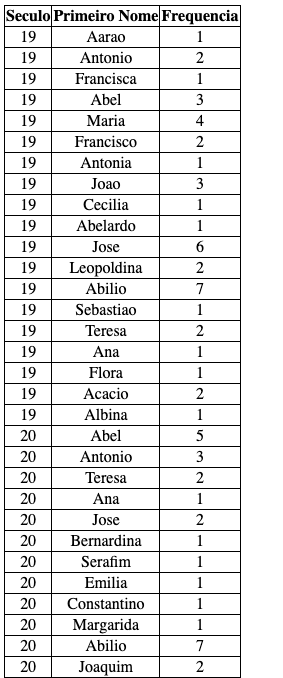
\includegraphics[height=3in]{freq_proprios_sec-tabela.png}
    \caption{Parte da Tabela de teste, Frequência de nomes próprios por século}
    \label{fig:my_label}
\end{figure}
\newpage
\subsubsection{Frequência de apelidos por século}
A abordagem a esta alínea é bastante similar à anterior.Aqui foi utilizada a expressão regular \textbf{r'([A-Za-z]+[ ])*([A-Za-z]+)($\backslash$,[A-Za-z]+)*', r'$\backslash$2'} que nos permite substituir o nome completo pelo apelido$\backslash$último nome. A última parte da expressão regular, \textbf{'($\backslash$,[A-Za-z]+)*'} é necessária devido a existirem apelidos seguidos de uma virgula e estado civil, "apelido,solteira". 
\begin{figure}[H]
    \centering
    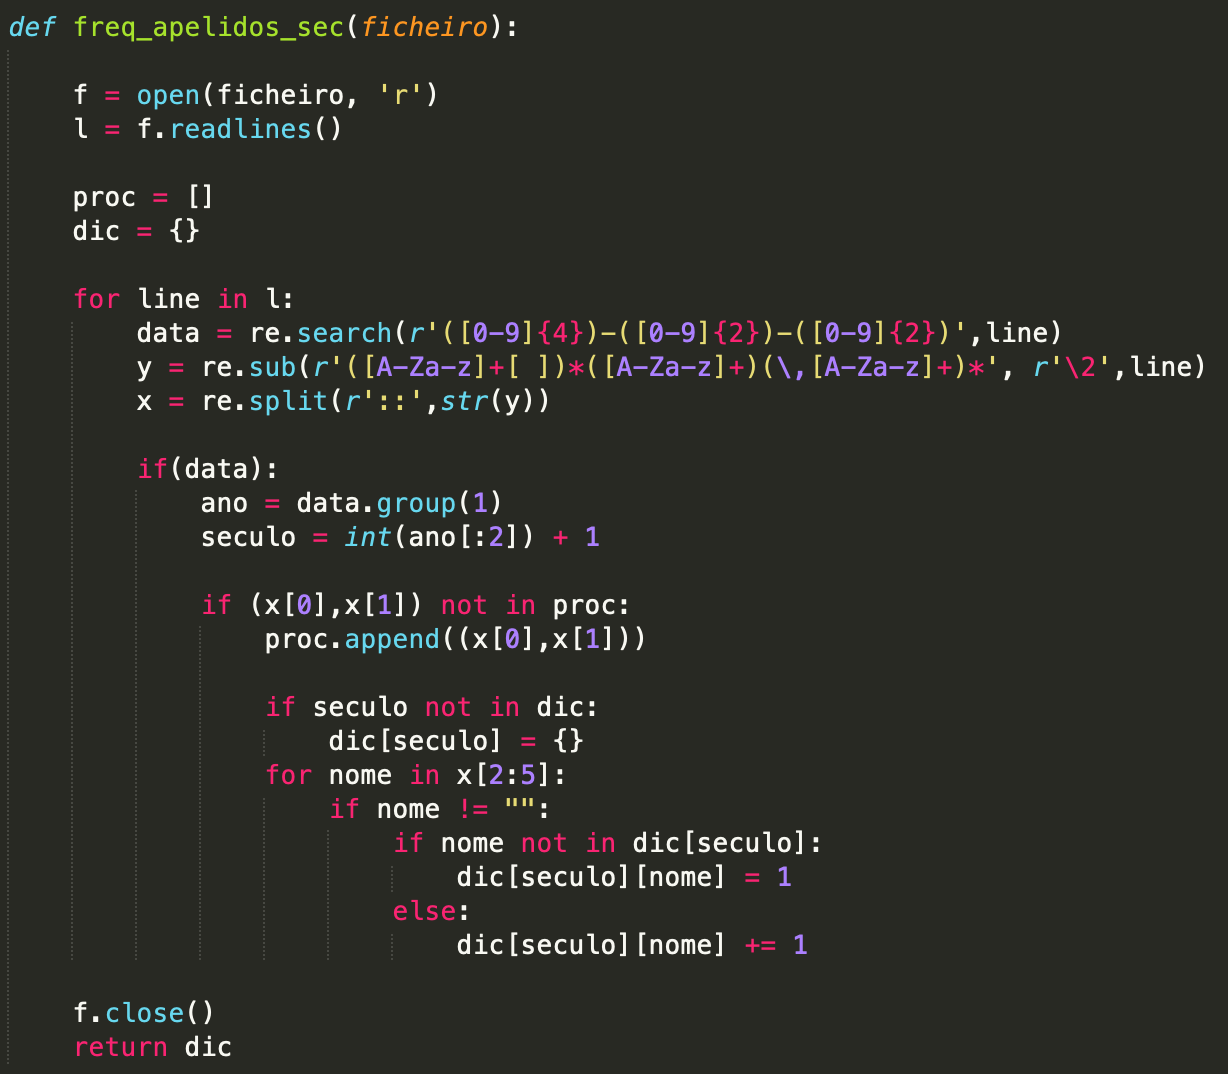
\includegraphics[height=3in]{freq_apelidos_sec.png}
    \caption{Frequência de apelidos por século}
    \label{fig:my_label}
\end{figure}
\begin{figure}[H]
    \centering
    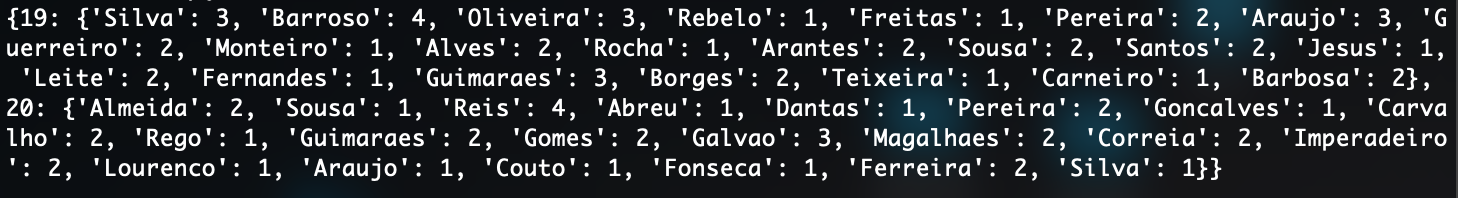
\includegraphics[height=0.5in]{freq_apelidos_sec-teste.png}
    \caption{Exemplo de teste, Frequência de apelidos por século}
    \label{fig:my_label}
\end{figure}
\begin{figure}[H]
    \centering
    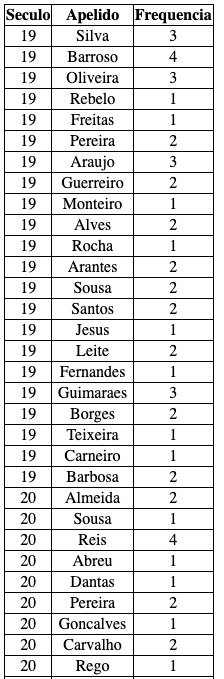
\includegraphics[height=3in]{freq_apelidos-tabela.png}
    \caption{Parte da Tabela de teste, Frequência de apelidos por século}
    \label{fig:my_label}
\end{figure}
\newpage
\subsection{Frequência dos tipos de relação}
Na resolução deste alínea foi usada a função \textbf{split()} associada ao caracter vírgula, pois as relações aparecem sempre entre uma virgula e um ponto final. Assim, foi iterado sobre o resultado anterior a partir da primeira virgula que aparece na linha e foi usada a função \textbf{match()} associada à expressão regular \textbf{'[A-Za-z]*($Irmao \vert Tio \vert Mae \vert Sobrinh[ao] \vert Pai \vert [nN]et[ao] \vert Meio \vert [Aa]vo$)[A-Za-z ]*$\backslash$.'} que nos permite encontrar todas as relações e devolver o último grupo do resultado que é o nome total da relação que está entre a virgula e o ponto final.
\begin{figure}[H]
    \centering
    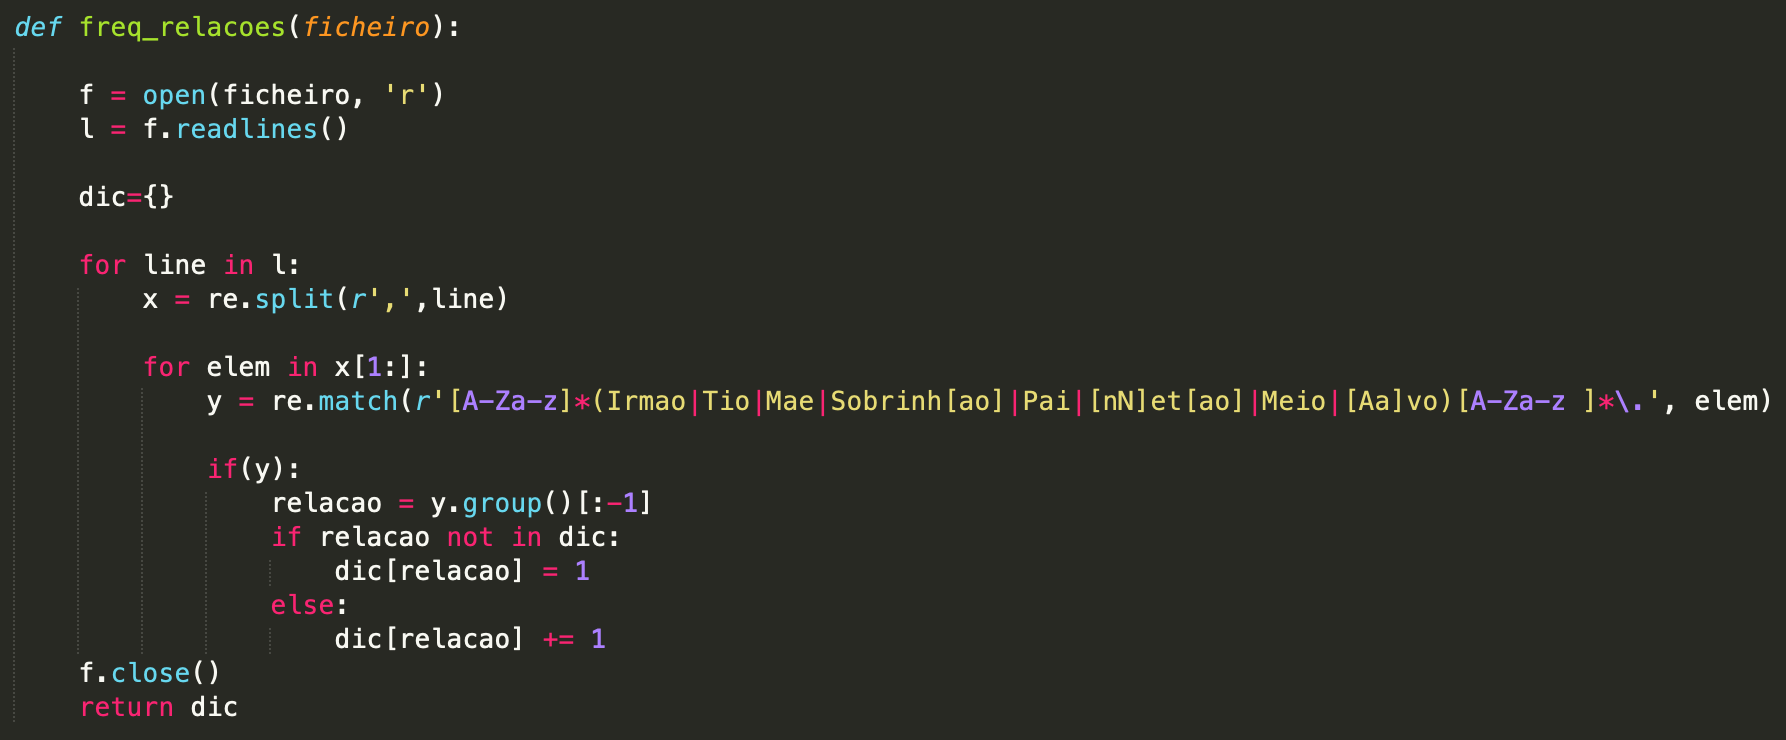
\includegraphics[height=2.5in]{freq_relacoes.png}
    \caption{Frequência de relações}
    \label{fig:my_label}
\end{figure}
\begin{figure}[H]
    \centering
    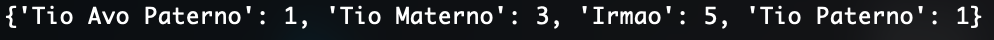
\includegraphics[height=0.2in]{freq_relacoes-teste.png}
    \caption{Exemplo de teste, Frequência de relações}
    \label{fig:my_label}
\end{figure}
\begin{figure}[H]
    \centering
    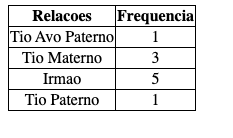
\includegraphics[height=2in]{freq_relacoes-tabela.png}
    \caption{Tabela de teste, Frequência de relações}
    \label{fig:my_label}
\end{figure}
\newpage
\subsection{Registos em formato Json}
Para imprimir em formato Json voltou a usar-se a função \textbf{split()} sobre as primeiras 20 linhas do ficheiro e criou-se um dicionário para cada linha que associa cada parâmetro do resultado anterior ao respetivo campo. Colocou-se os dicionários todos numa lista e gerou-se o ficheiro Json.Devido ao ficheiro Json ser extenso, apenas é mostrado parte do mesmo.
\begin{figure}[H]
    \centering
    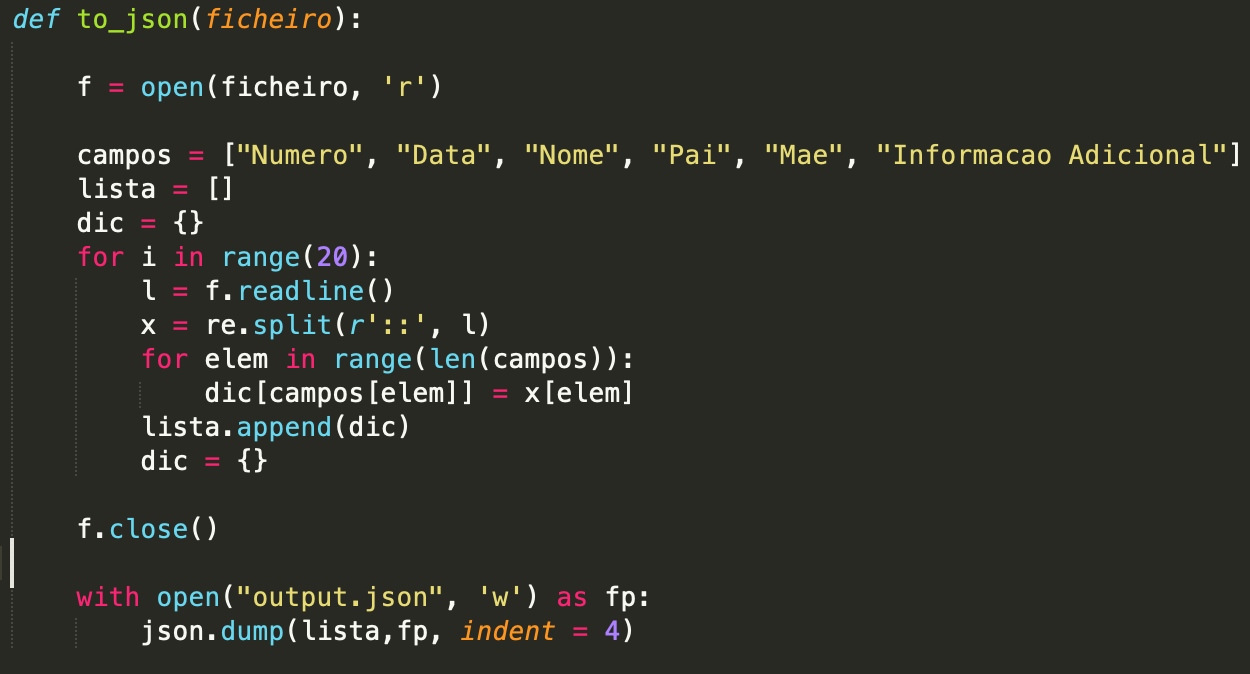
\includegraphics[height=2in]{Captura de ecrã 2022-10-29, às 00.56.50.png}
    \caption{Conversão para Json}
    \label{fig:my_label}
\end{figure}
\begin{figure}[H]
    \centering
    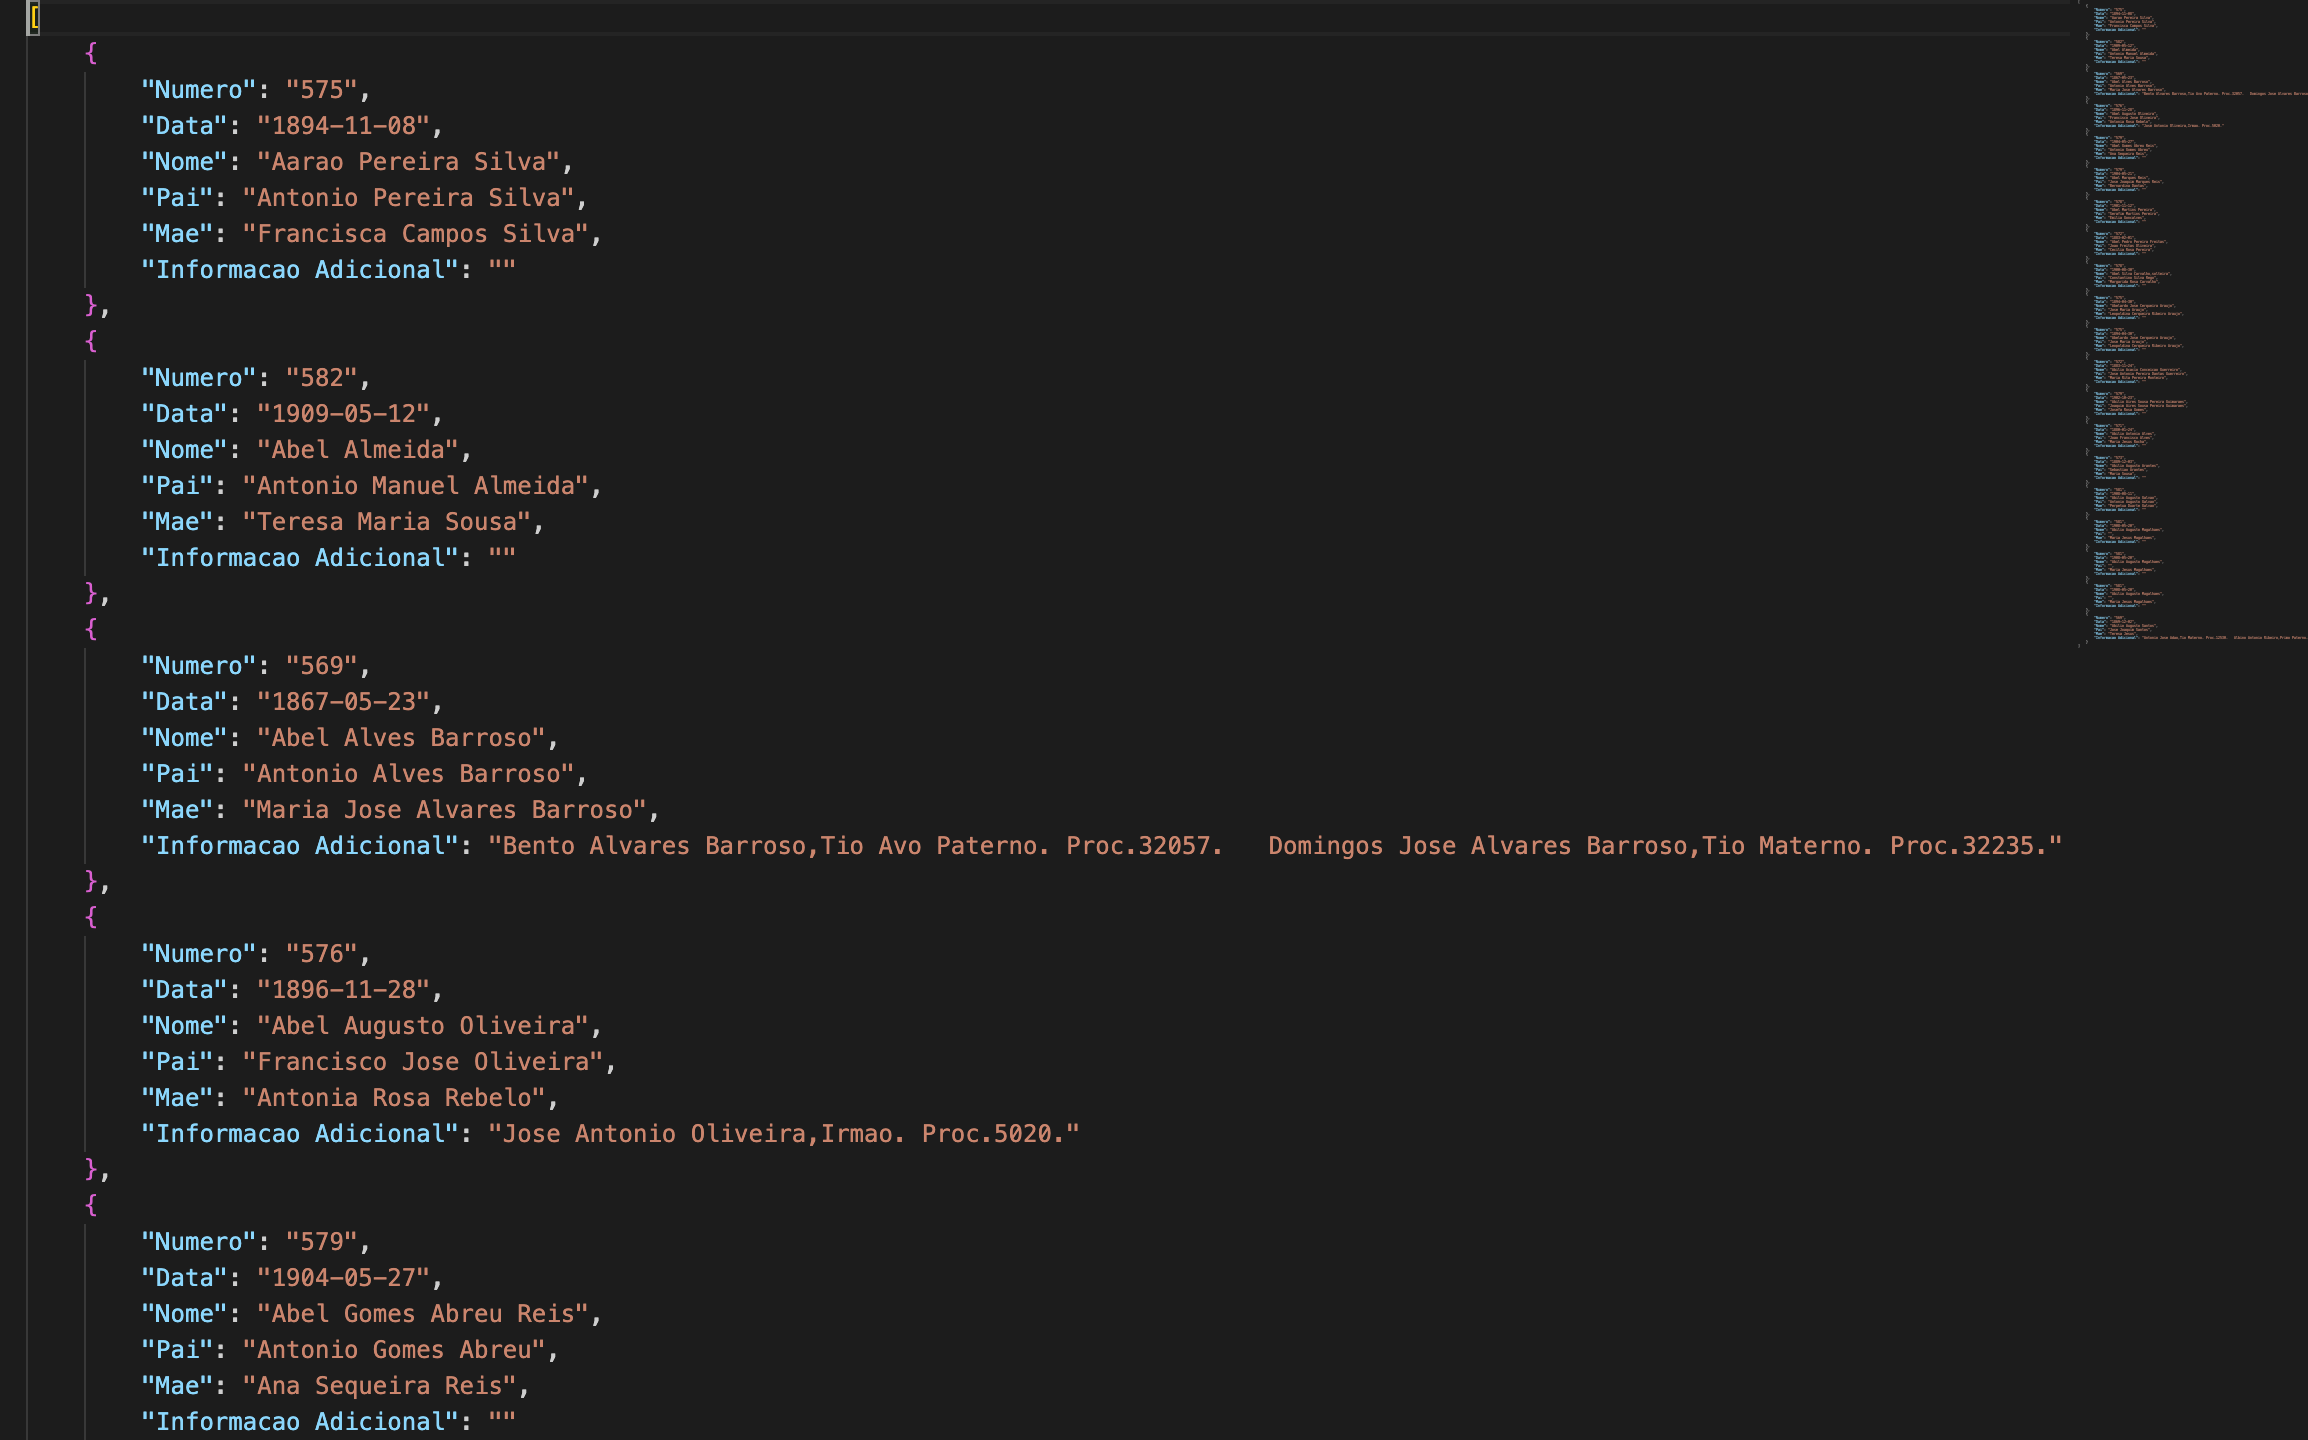
\includegraphics[height=2in]{to_json-teste.png}
    \caption{Exemplo de teste, Conversão para Json}
    \label{fig:my_label}
\end{figure}
\newpage
\section{Análise de resultados Processos.txt}
Nesta seccção, irei mostrar os resultado das funções aplicadas ao ficheiro processos.txt. Em alguns casos, devido ao facto de o resultado ser muito extenso apenas irei mostrar parte do mesmo.
\subsection{Frequência de processos por ano}
Parte do dicionário e da tabela que asscociam a cada ano o número de processos.
\begin{figure}[H]
    \centering
    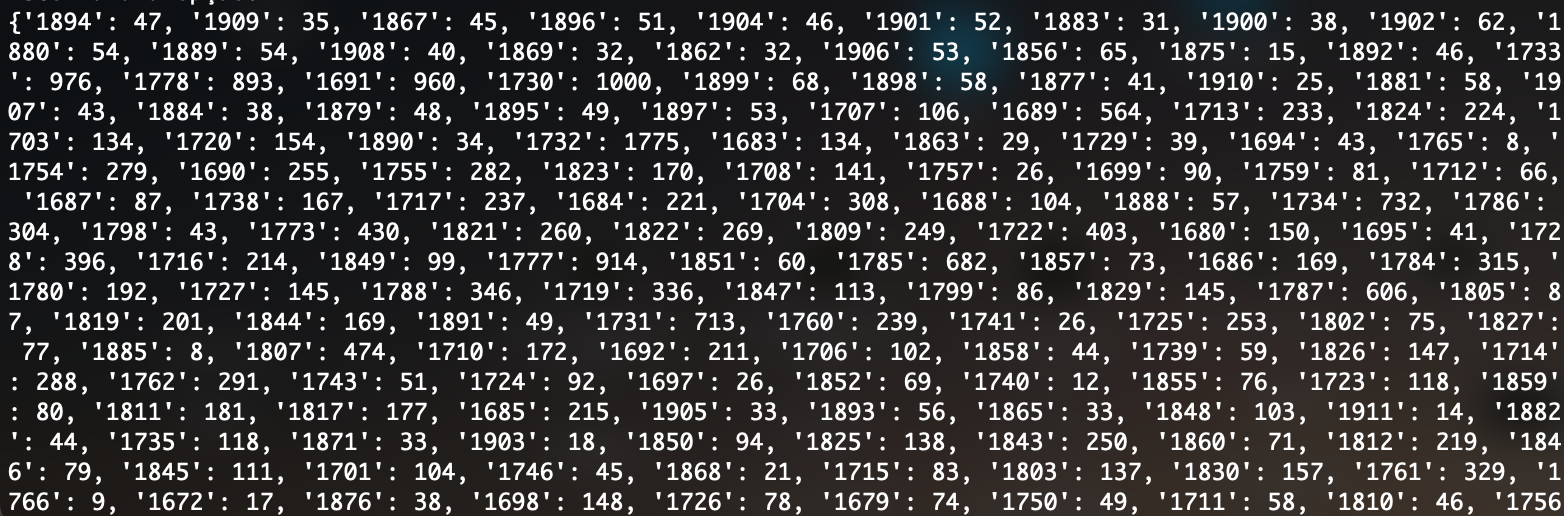
\includegraphics[height=1.5in]{1.png}
    \caption{Frequência de processos por ano}
    \label{fig:my_label}
\end{figure}
\begin{figure}[H]
    \centering
    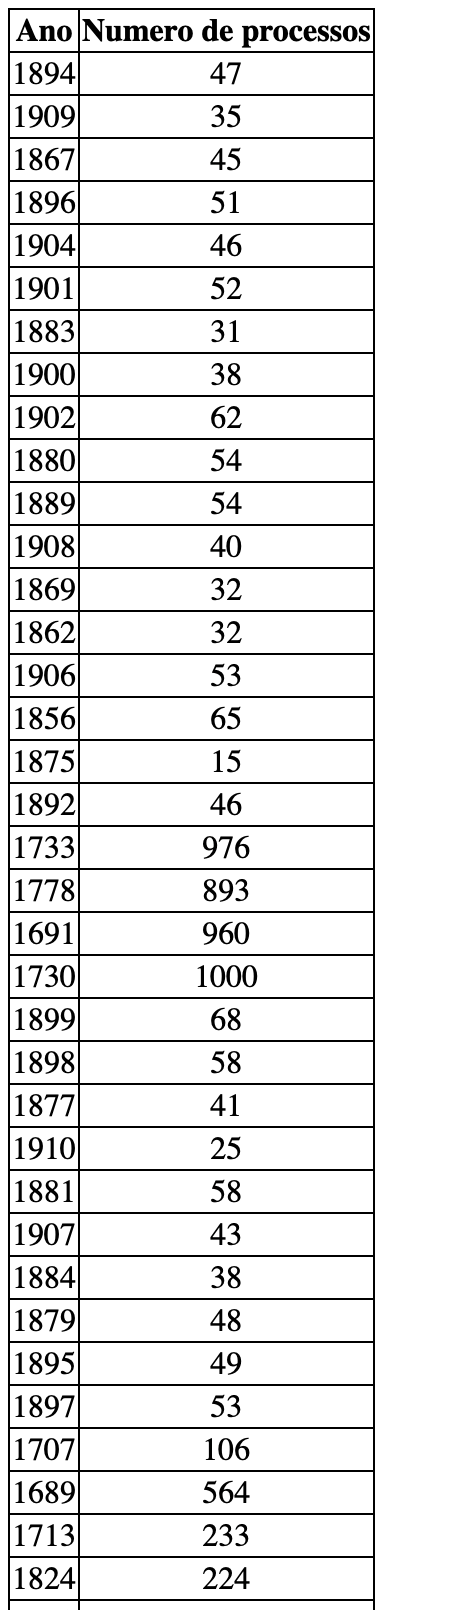
\includegraphics[height=3in]{1-tabela.png}
    \caption{Tabela, Frequência de processos por ano}
    \label{fig:my_label}
\end{figure}
\newpage
\subsection{Frequência de nomes próprios por século}
Parte do dicionário e da tabela que associam a cada século os nomes próprios que ocorrem e a respetiva frequência.
\begin{figure}[H]
    \centering
    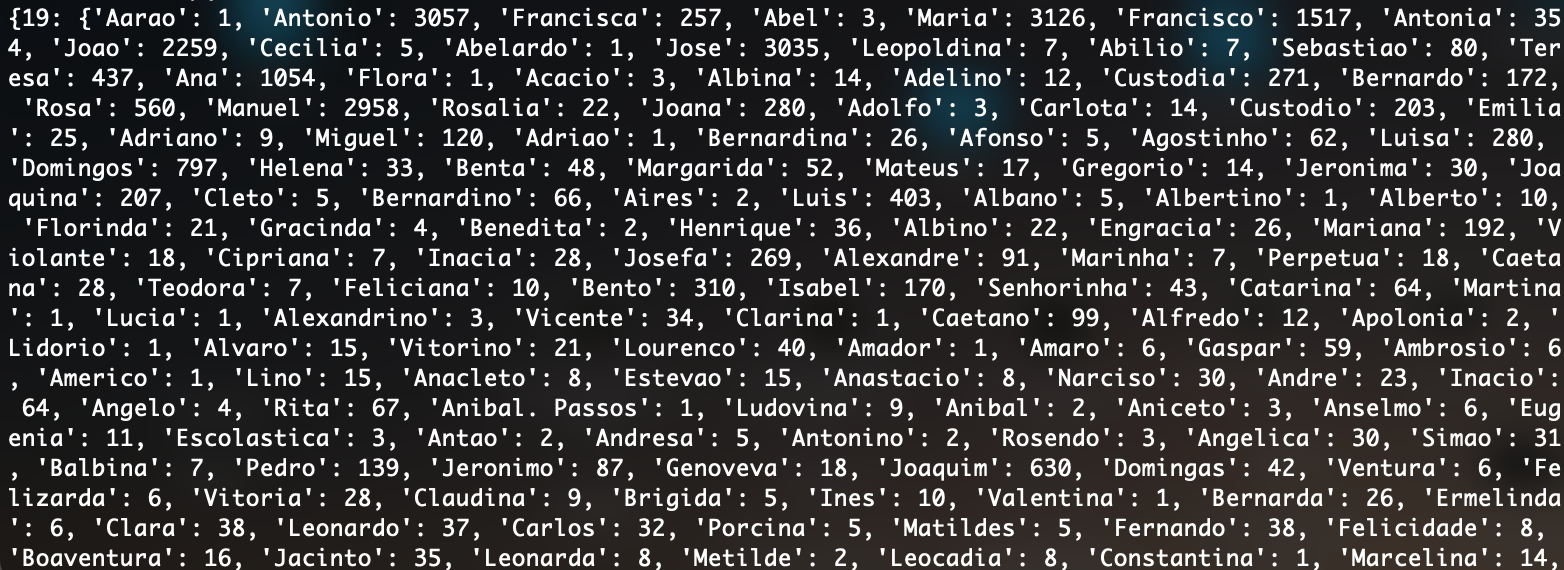
\includegraphics[height=1.5in]{2.png}
    \caption{Frequência de nomes próprios por século}
    \label{fig:my_label}
\end{figure}
\begin{figure}[H]
    \centering
    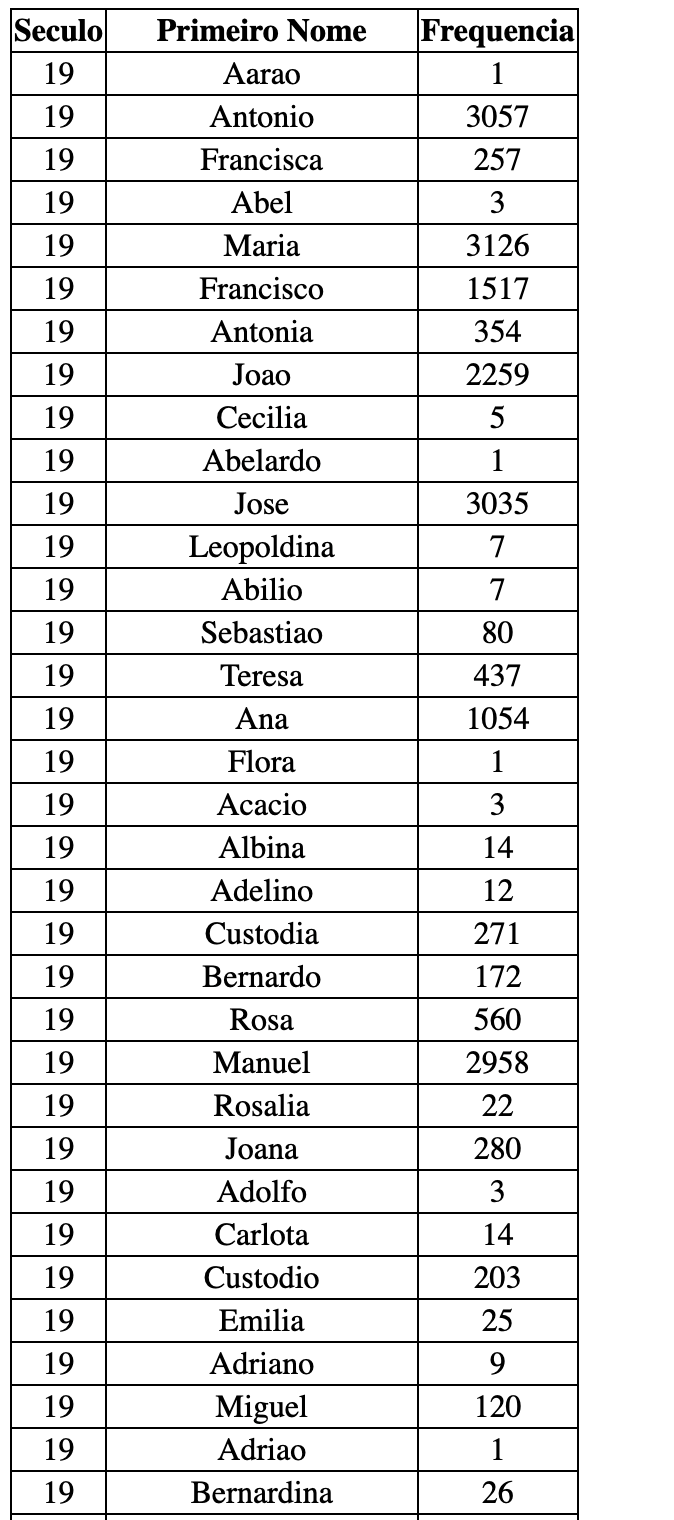
\includegraphics[height=3in]{2-tabela.png}
    \caption{Tabela, Frequência de nomes próprios por século}
    \label{fig:my_label}
\end{figure}
\newpage
\subsection{Frequência de apelidos por século}
Parte do dicionário e da tabela que associam a cada século os apelidos que ocorrem e a respetiva frequência.
\begin{figure}[H]
    \centering
    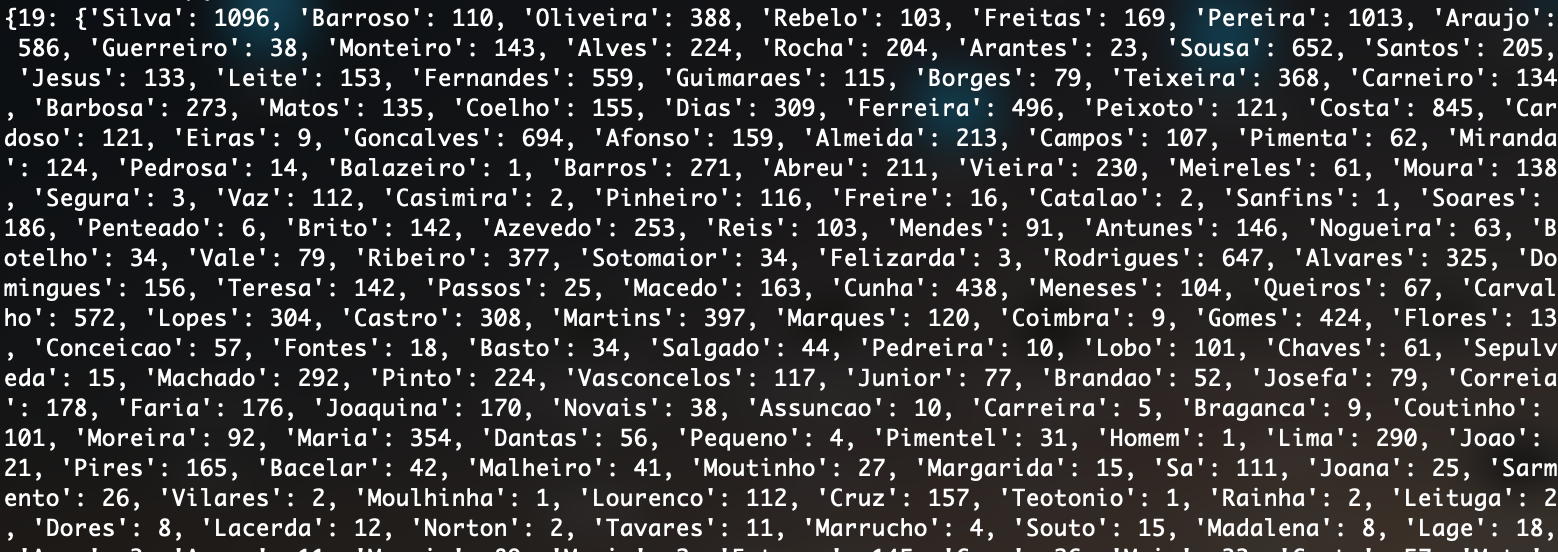
\includegraphics[height=1.5in]{3.png}
    \caption{Frequência de apelidos por século}
    \label{fig:my_label}
\end{figure}
\begin{figure}[H]
    \centering
    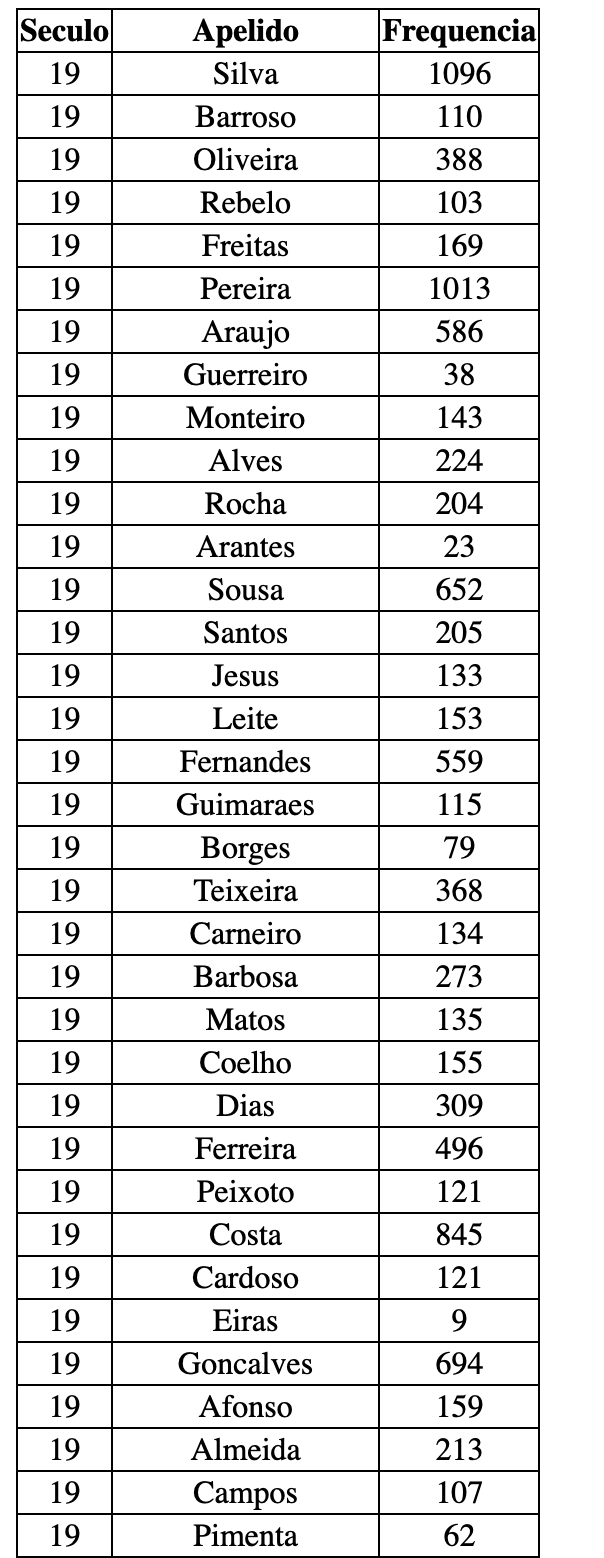
\includegraphics[height=3in]{3-tabela.png}
    \caption{Tabela,Frequência de apelidos por século}
    \label{fig:my_label}
\end{figure}
\newpage
\subsection{Frequência de relações}
Dicionário e tabela com o número de frequência das relações.
\begin{figure}[H]
    \centering
    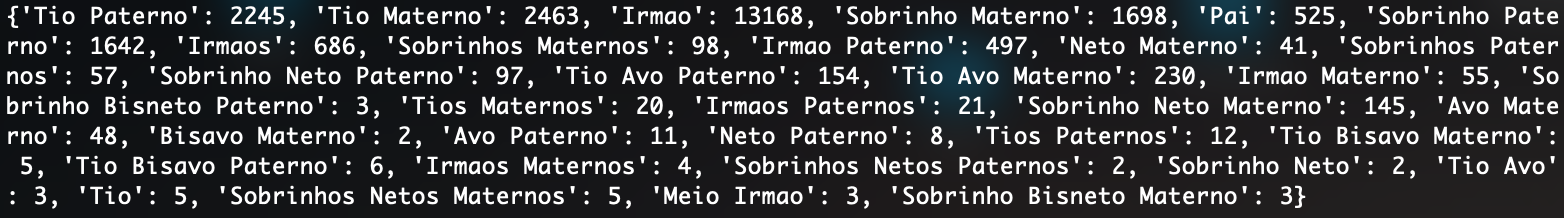
\includegraphics[height=0.8in]{4.png}
    \caption{Frequência de relações}
    \label{fig:my_label}
\end{figure}
\begin{figure}[H]
    \centering
    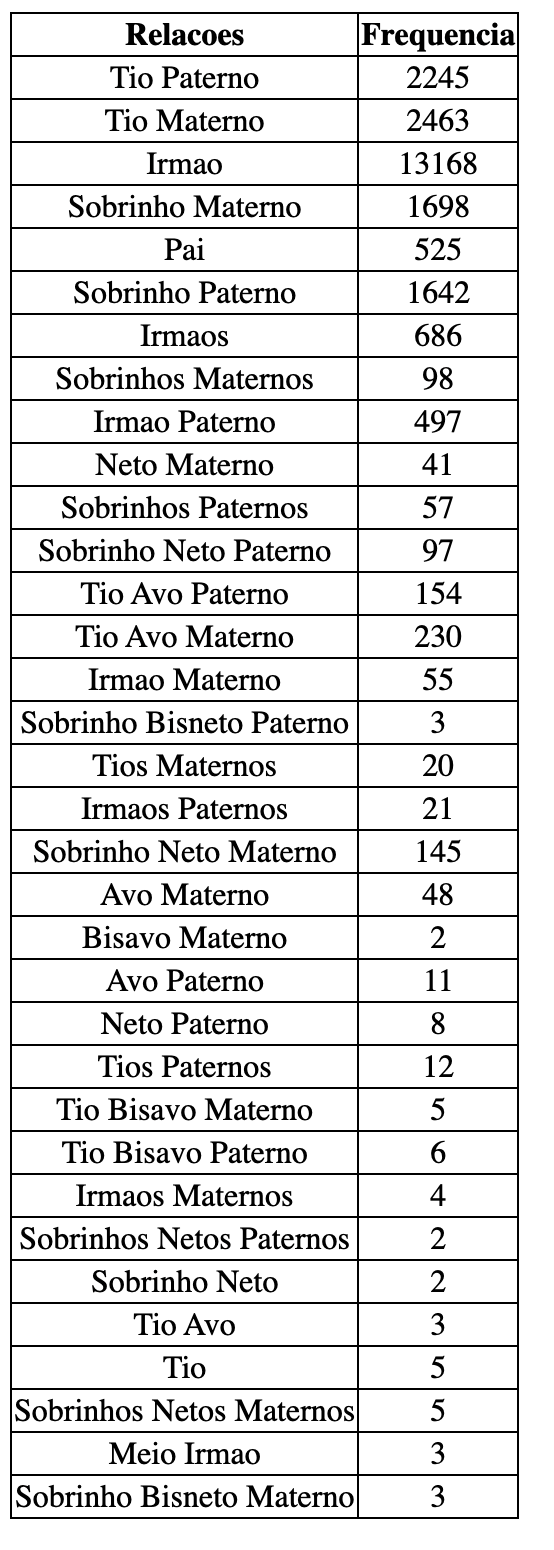
\includegraphics[height=3in]{4-tabela.png}
    \caption{Tabela, Frequência de relações}
    \label{fig:my_label}
\end{figure}
\newpage
\section{Conclusão}
Com a realização deste trabalho, os objetivos esperados foram alcançados e a experiência na manipulação de expressões regulares aumentou.

A elaboração do projeto contribui para o desonlvimento de código em linguagem HTML e para o aumento da experiência relativamente a uma forma de armazenamento de dados e representação, o Json.

O desenvolvimento do relátorio em LaTex permitiu ainda aumentar o conhecimento sobre este sitema de edição de documentos.







\newpage
\section{Código dos ficheiros}
\subsection{Ficheiro func.py}
O ficheiro \textbf{fun.py} é constituido pelo código mostrado na resolução das alíneas e pelas funções que transformam um dicionário em um ficheiro HTML seguintes:
\begin{figure}[H]
    \centering
    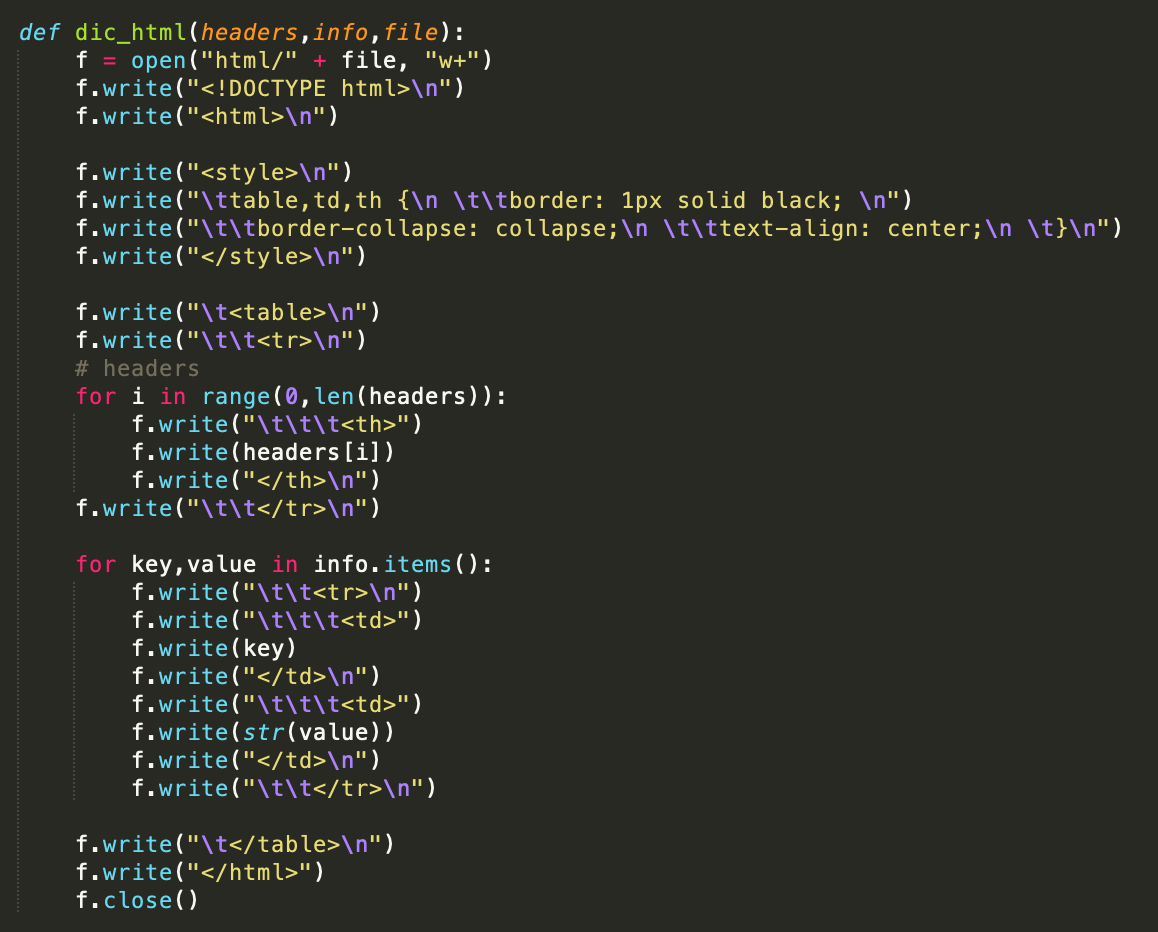
\includegraphics[height=4in]{dic1.png}
    \caption{Dicionário Python para HTML}
    \label{fig:my_label}
\end{figure}
\begin{figure}[H]
    \centering
    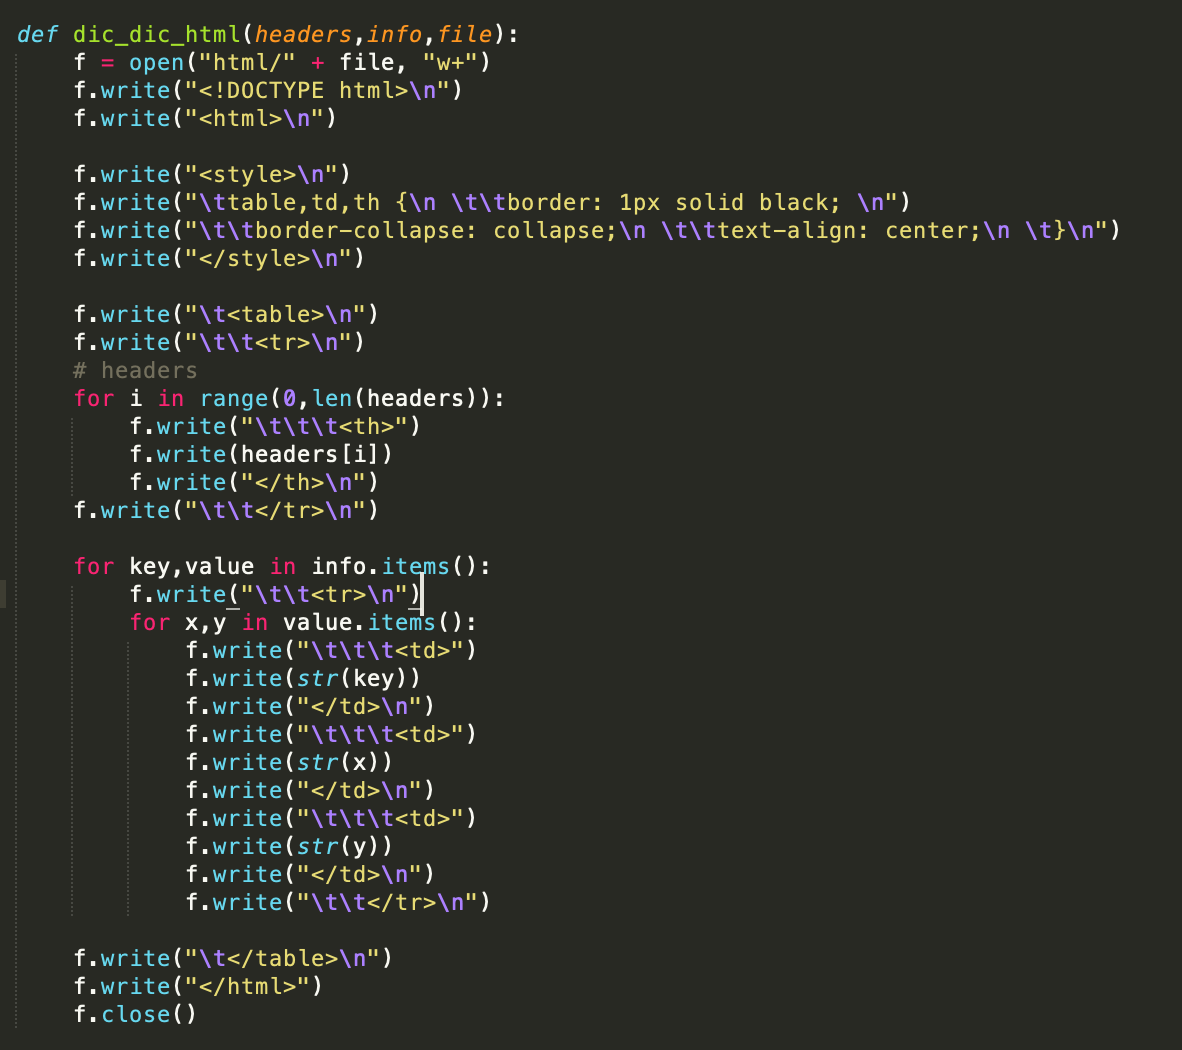
\includegraphics[height=4in]{dicdic.png}
    \caption{Aninhamento de dicionários Python para HTML}
    \label{fig:my_label}
\end{figure}
\newpage
\subsection{Ficheiro main.py}
O ficheiro \textbf{main.py} é constituído pelo código relativo à implementação do menu e invocação das funções.
\begin{figure}[H]
    \centering
    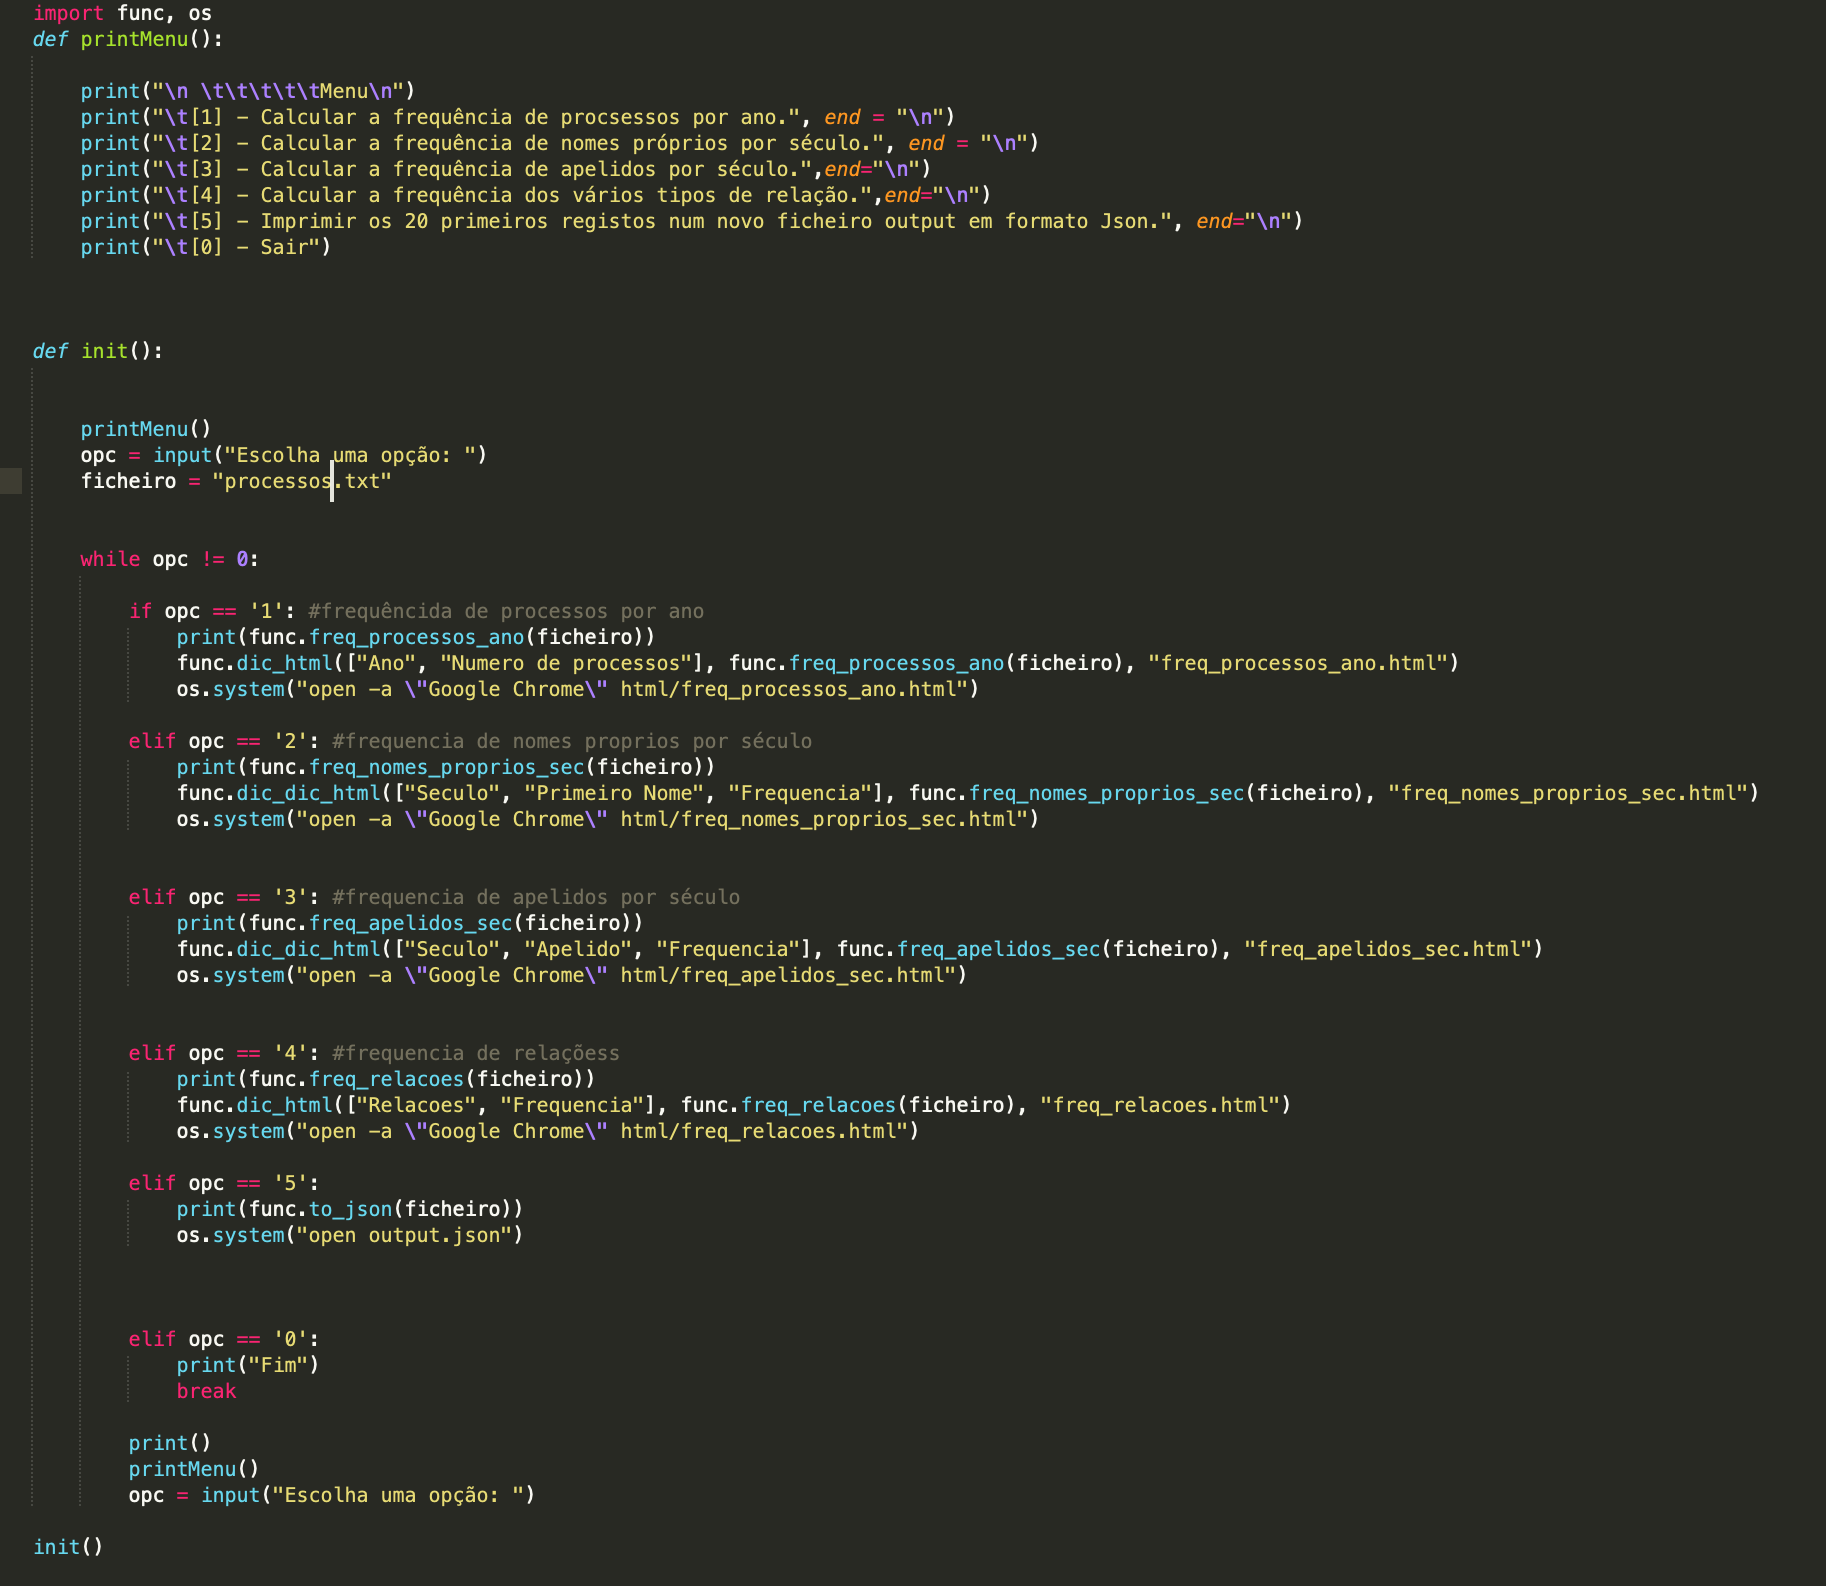
\includegraphics[height=5in]{mennu.png}
    \caption{Código ficheiro main.py}
    \label{fig:my_label}
\end{figure}
\end{document}



